
\documentclass[10pt,letterpaper]{article}



% Some useful packages
% math
\usepackage{amsmath}
\usepackage{amsfonts}
\usepackage{algorithm}
\usepackage[noend]{algpseudocode}
\usepackage{amssymb}
% pretty colors
\usepackage{color}
% nicer urls that break at the end of the page
\usepackage{url}
% every document needs images
\usepackage{graphicx}
\usepackage{setspace}

\newcommand{\e}[1]{\mathbb E}
\newcommand{\R}{\mathbb{R}}
\newcommand\given[1][]{\:#1\vert\:}
\DeclareMathOperator*{\argmin}{arg\,min} % thin space, limits underneath in displays
\DeclareMathOperator*{\argmax}{arg\,max} % thin space, limits underneath in displays
\newcommand{\var}[1]{{\operatorname{\mathit{#1}}}}

\graphicspath{{./figures/}}   % where to look for images

%let's fiddle with the default margins to save some trees
%this makes the odd side margin go to the default of 1inch
\oddsidemargin 0.0in
%sets the textwidth to 6.5, which leaves 1 for the remaining right margin with 8 1/2X11inch paper
\textwidth 6.5in
% less white space, please!
\headheight 0.0in
% shift everything up
\topmargin -0.5in
\footskip .6in
% text should take up all but a 1'' margin
\textheight 9.0in

% Define some shortcuts for things I want to use.
% Use them like, for example:
% \begin{hypothesis}Lettuce causes brain damage.\end{hypothesis}
% Numbering & formatting will happen automatically.
\newtheorem{hypothesis}{Hypothesis}
\newtheorem{task}{Task}
\newtheorem{contribution}{Contribution}


% Shortcuts: allows you to use limited markup when editing/collaborating.
% \comment{This section needs to be rewritten.}
\def\ask#1{\textcolor{red}{\bf $\langle\langle$Question:\ #1$\rangle\rangle$}}
\def\comment#1{\textcolor{red}{\bf $\langle\langle$Comment:\ #1$\rangle\rangle$}}


% This imitates the Wikipedia ``Citation Needed'' text; use it as a temporary
% marker for things you need to cite.
\def\citationneeded{$^{\textcolor{blue}{\text{[citation needed]}}}$ }

% format et al.
\def\etal{\textit{et al.}}
\def\ie{\textit{i.e.}}
\def\eg{\textit{e.g.}}

\title{Attempts to exercise in Reinforcement Learning book Chapter 4}
\author{Mengliao Wang}


\begin{document}

% Generate Title Page
\maketitle


% this dumps the abstract on a front page all by itself.

\section*{Exercise 4.1: }
\label{4.1}

According to $q_\pi(s,a) = r(s,a,s') + \gamma\sum_{s',r}p(r,s'\given s,a)v_\pi(s')$

We have $q_\pi(11, down) = -1 + v(T) = -1$.

Similarly we have $q_\pi(7, down) = -1 + v(11)$. Here $v(11)$ would take iterations to calculate, but given enough runs, it will converge to $-14$ as shown in Figure 4.1. Thus the optimal action value $q_\pi(7, down) = -15$.

\section*{Exercise 4.2: }
\label{4.2}

If the dynamic of original states are unchanged, then $v_\pi(s), s=1,2,..,14$ will not be changed. So we have value function 

\begin{align}
v_\pi(15) &= 0.25\times[-1 + v_\pi(12)] + 0.25\times[-1 + v_\pi(13)]  + 0.25\times[-1 + v_\pi(14)] + 0.25\times[-1 + v_\pi(15)]\\
&= 0.25\times(-23) + 0.25\times(-21)  + 0.25\times(-15) + 0.25\times[-1 + v_\pi(15)]
\end{align}
By solving the equation above we have $v_\pi(15) = -20$.

If grid 13 will go down to the new grid 15, then we have the following equations:
\begin{align}
v_\pi(15) &= 0.25\times[-1 + v_\pi(12)] + 0.25\times[-1 + v_\pi(13)]  + 0.25\times[-1 + v_\pi(14)] + 0.25\times[-1 + v_\pi(15)]\\
&= 0.25\times(-23) + 0.25\times(-1 + v_\pi(13))  + 0.25\times(-15) + 0.25\times[-1 + v_\pi(15)]\\
&= -10 + 0.25\times[v_\pi(13) + v_\pi(15)]\\
v_\pi(13) &= 0.25\times[-1 + v_\pi(12)] + 0.25\times[-1 + v_\pi(9)]  + 0.25\times[-1 + v_\pi(14)] + 0.25\times[-1 + v_\pi(15)]\\
&= 0.25\times(-23) + 0.25\times(-21)  + 0.25\times(-15) + 0.25\times[-1 + v_\pi(15)]\\
&= -15 + 0.25\times v_\pi(15)
\end{align}

By resolving the equations above we still have $v_\pi(15) = v_\pi(13) = -$.

\section*{Exercise 4.3: }
\label{4.3}

Equation 4.3, 4.4 for $q_\pi(s,a)$ is:

\begin{align}
q_\pi(s,a) &= \mathbb{E}[R_{t+1} + \gamma v_\pi(s') \given S_t=s, A_t=a]\\
&= \mathbb{E}[R_{t+1} + \gamma \mathbb{E}_\pi[q_\pi(s',a')] \given S_t=s, A_t=a, S_{t+1} = s']\\ 
&= r + \gamma\sum_{s',r}p(s',r\given s,a)\sum_{a'}\pi(a'\given s')q_\pi(s', a')
\end{align}

So we can have the approximation for $q_\pi(s,a)$ as:

\begin{align}
q_{k+1}(s,a) &= r + \gamma\sum_{s',r}p(s',r\given s,a)\sum_{a'}\pi(a'\given s')q_{k}(s', a')
\end{align}


\section*{Exercise 4.4: }
\label{4.4}

First of all, if a policy will have non-zero probablities for all the actions given any state, then we will not have this issue. The negative infinity value only happens when certain states consist of a subset S', with no transition between the remaining states S-S'. To avoid this issue we can introduce some of the approaches explained in Chapter 2, such as an exploration rate $\epsilon$.

To be more specific, in the algorithm while update $V(s)$, we can update it to:

\begin{center}
\[V(s) \leftarrow \begin{cases}
\sum_a\pi(a|s)\sum_{s',r}p(s',r\given s,a)[r+\gamma V(s')], & \text{with probability } 1-\epsilon \\
\sum_a\pi'(a|s)\sum_{s',r}p(s',r\given s,a)[r+\gamma V(s')], & \text{with probability } \epsilon
\end{cases}
\]
\end{center}

Here $\pi'$ is any non-zero policy, such as random equiprobable policy.

\section*{Exercise 4.5: }
\label{4.5}

\begin{figure}[htp]
  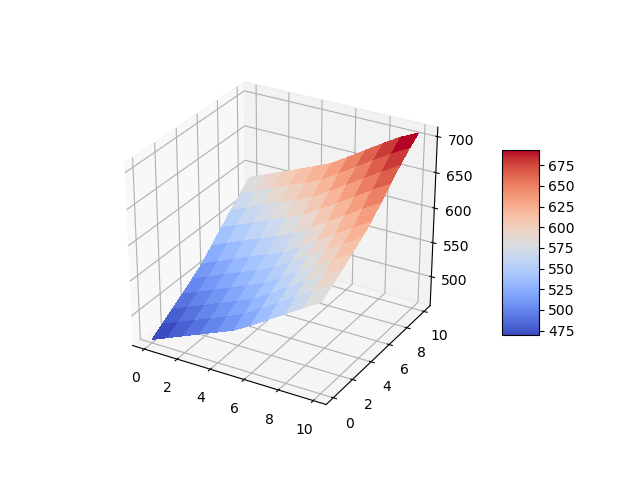
\includegraphics[width=.5\textwidth]{Car_rental_Value}
  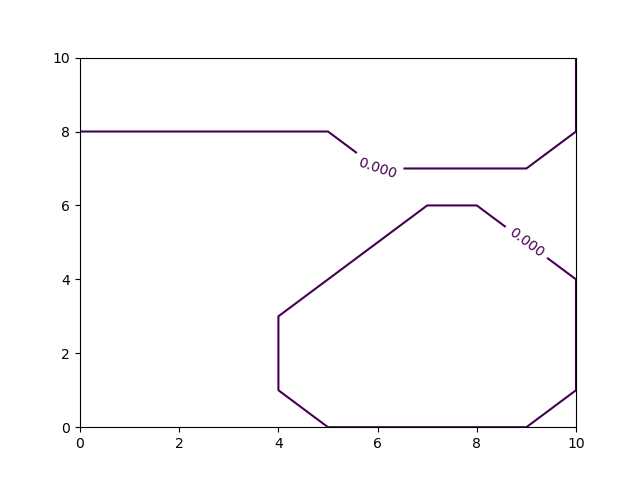
\includegraphics[width=0.5\textwidth]{Car_rental_Policy}
  \caption{Value and Policy for Exercise 4.5 solution with 10 maximum cars per location, and 5 maximum free parking}
  \label{fig:car-rental}
\end{figure}

Python code attached. I cut the maximum number of cars to be 10 and the parking limit to be 5. Figure \ref{fig:car-rental} is the optimal value and policy for the problem.

\section*{Exercise 4.6: }
\label{4.6}

\begin{algorithmic}
\State 1. Initialization: 
\State $Q(s, a) \in \R$ and $\pi(s) \in A(s)$ arbitrarily for all $s \in S$ and $a \in A(s)$
\State
\State 2. Policy Evaluation:
\Repeat
    \State $\Delta \gets 0$
    \For {Each $s \in S$:}
	\For {Each $a \in A(s)$:}
	\State $q \gets Q(s, a)$
	\State $Q(s,a) \gets r(s,a) + \gamma\sum_{s',r}p(s',r|s,a)\sum_{\pi(s')}\pi(s')Q(s',\pi(s'))$
	\State $\Delta \gets \max(\Delta, |q-Q(s,a)|$)
	\EndFor
    \EndFor
\Until{$\Delta < \theta$ (a small positive number)}
\State
\State 3. Policy Improvement:
\State $\var{policy-stable} \gets true$
\For {each $s \in S$:}
\State $\var{old-action} \gets \pi(s)$
\State $\pi(s) \gets \argmax_aQ(s,a)$
\If {$\var{old-action} \neq \pi(s)$}
\State $\var{policy-stable} \gets false$
\EndIf
\EndFor
\If {$\var{policy-stable}$}
\State stop and return $Q\approx q_*$
\Else
\State go to 2
\EndIf

\end{algorithmic}

\section*{Exercise 4.7: }
\label{4.7}

For step 3 in the algorithm, For each state instead of assigning a single value, we will need to assign probability for each state-action pair $\pi(s,a)$. For action that maximize $\sum_{s',r}p(s',r|s,a)[r+\gamma V(s')]$, $\pi(s,a) = 1 - \epsilon + \dfrac{\epsilon}{|A(s)|}$. For all the other actions $\pi(s,a) = \dfrac{\epsilon}{|A(s)|}$. Everything else would stay the same, except that the old-action would be a array with all the probabilities under s, i.e. $\pi(s, ...)$

For step 2 in the step that update $V(s)$, we need to loop through all the actions under state s, and reset $V(s)$ to be 0 after $v \gets V(s)$. Then for each action loop, we define $V(s) \gets V(s) + \pi(s,a)\sum_{s',r}p(s',r|s,a)[r+\gamma V(s')]$. Everything else stays the same.

For step 1 $V(s)$ does not change. But we need to make $\pi(s)$ to be a matrix $\pi(s,a), a \in A(s)$. Also for initialization we must make sure $\pi(s,a) > \epsilon, \forall s,a$ and $\sum_a(s,a) = 1, \forall s \in S$


\section*{Exercise 4.8: }
\label{4.8}

What caused this form is the fact that the value function for mid point $v(50)$ is slightly higer than the regression curve, due to the fact that the value $v(50)$ is deterministic of 0.4. Thus the other states will prefer to take actions to move to this state, e.g. at state 51 it will take action = 1, at state 25/75 it will take action = 25, etc.. Based on the same reason state 50 itself will prefer deterministic destination states, i.e. state 0 and 100. Thus it will bet all on the flip.


\section*{Exercise 4.9: }
\label{4.9}

\begin{figure}[htp]
  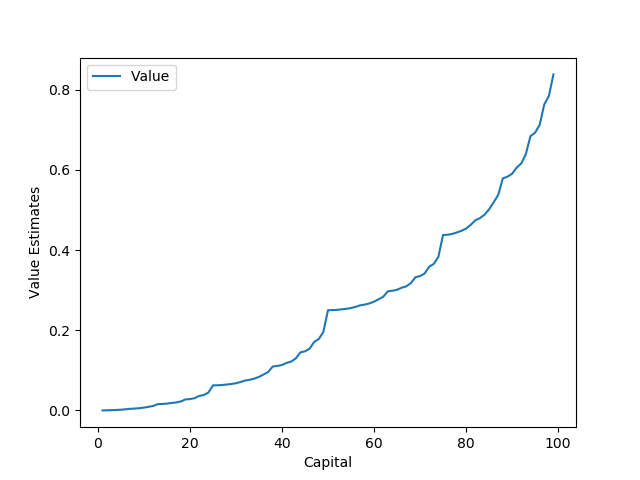
\includegraphics[width=.5\textwidth]{Gambler_p_0_25_value}
  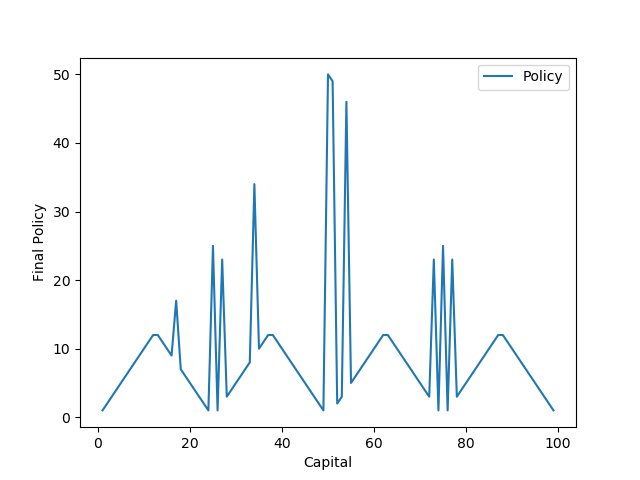
\includegraphics[width=0.5\textwidth]{Gambler_p_0_25_policy}
  \caption{Final value and policy for Gambler with $p_h = 0.25$}
  \label{fig:gambler_25}
\end{figure}

\begin{figure}[htp]
  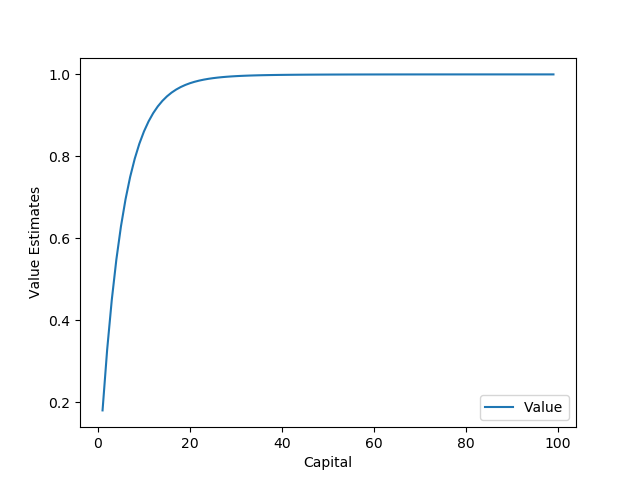
\includegraphics[width=.5\textwidth]{Gambler_p_0_55_value}
  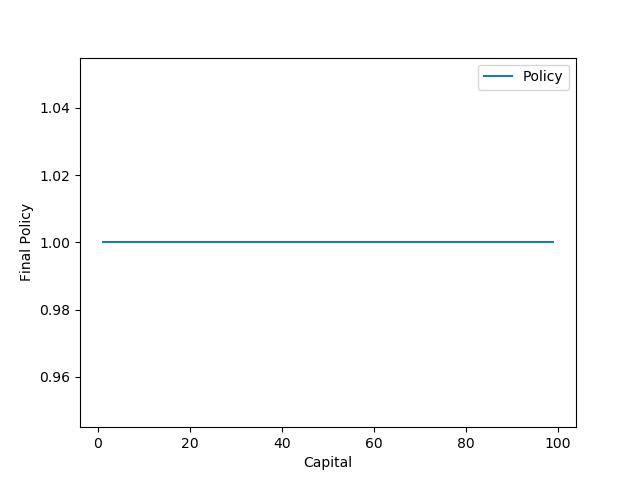
\includegraphics[width=0.5\textwidth]{Gambler_p_0_55_policy}
  \caption{Final value and policy for Gambler with $p_h = 0.55$}
  \label{fig:gambler_55}
\end{figure}


Python program attached. I was unable to reproduce the optimal policy shown in Figure 4.3 in the book for $p_h=0.4$, But after debugging I believe that is due to the approximation. Figure \ref{fig:gambler_25} and Figure \ref{fig:gambler_55} show the final optimal value and policy for $p_h = 0.25$ and $p_h = 0.55$ respectively.


\section*{Exercise 4.10: }
\label{4.10}
Obviously we have:
\begin{align}
q_{k+1}(s,a) = \sum_{s',r}p(s',r\given s,a)[r + \gamma\max_aq_k(s,a)]
\end{align}

\clearpage

\end{document}
